\chapter{$Z\to\tauh\taul$ tag and probe study}\label{chap1}
This chapter describes the analysis methodology of using $Z\to\tau\tau$ events to measure Monte Carlo correction factors for tau identification algorithms on the high-$p_T$ region.

As we saw in the previous section different working points are defined for RNN score relative to the efficiency of selecting true $\tauh$ candidates. When the efficiency of the working points is measured in data and simulation, a correction factor is derived and then applied to the simulation in order for the signal efficiency to agree between data and simulation REF TAU ID PERFORMANCE. Because of the top quark mass, $t\bar{t}$ events are used as a source of high momentum taus for measuring correction factors on the high-$p_T$ bins. But as we already saw in section \ref{chap2sec2}, LU may not hold on W decays. For that reason our study is aimed to use $Z\to\tau\tau$ events for deriving simulation correction factors on the high-$p_T$ region.   

\section{Signal events}
The type of $Z\to\tau\tau$ events that we will consider as signal are when one of the taus decays hadronically and the other leptonically either into an electron or a muon ($Z\to\tau\tau\to\tau_h +l=\mu,e$). Thus, our final states will include a $\tauh$ candidate and a lepton $l=e,\mu$. The presence of this lepton will be used as our tag. 
Generally, in $Z\to\tau\tau$ events, the taus are produced back to back and their $\pt$ spectrum is does not go very high. One way to select events where the taus are boosted on the transverse plain is to look for events where the opening angle in the transverse plane between the taus ($\Delta\phi(\tauh,\taul)$) is more acute. For these events, the missing transverse momentum ($\ptmiss$) is assumed to come from the neutrinos produced in the decays of the tau leptons. Due to the fact that two neutrinos are produced in the leptonic decay mode we expect our events to have a larger $\ptmiss$ component along the $\taul$ direction.

We classify our events in two types of topologies. First, events where the $\ptmiss$ is inside the opening angle between the visible objects, in this kind of events we assume the missing energy is due to a pair of neutrinos flying in the same direction as the visible objects. This is shown in Fig.\ref{Fig7a} . In this case we solve the following equation to obtain the momentum of the neutrinos:
\begin{align}
	\vec{p}_{T_{\nu_l}}+\vec{p}_{\nu_h}&=\vec{p}_{T_{\text{miss}}},
	\\
	\phi(\nu_l)&=\phi(l),
	\\
	\phi(\nu_h)&=\phi(\tauh),
	\\
	\eta(\nu_l)&=\eta(l),
	\\
	\eta(\nu_h)&=\eta(\tauh).
\end{align}
The second case is when the $\ptmiss$ is outside the angle formed by the visible objects, as is shown in Fig.\ref{Fig7b}, in this case the assumption is that only one neutrino is responsible for the majority of the $\ptmiss$, a neutrino flying in the direction of the visible particle that is closer to the $\ptmiss$. We solve the following equations to obtain the neutrino momentum:
\begin{align}
p_{T_{\nu}}&=\ptmiss \cos(\Delta\phi(\tau_{\text{closer}},\ptmiss)),
\\
\phi(\nu)&=\phi(\tau_{\text{closer}}),
\\
\eta(\nu)&=\eta(\tau_{\text{closer}}),
\end{align} 
\begin{figure}[ht]
	\centering
	\subfloat[]{\label{Fig7a}{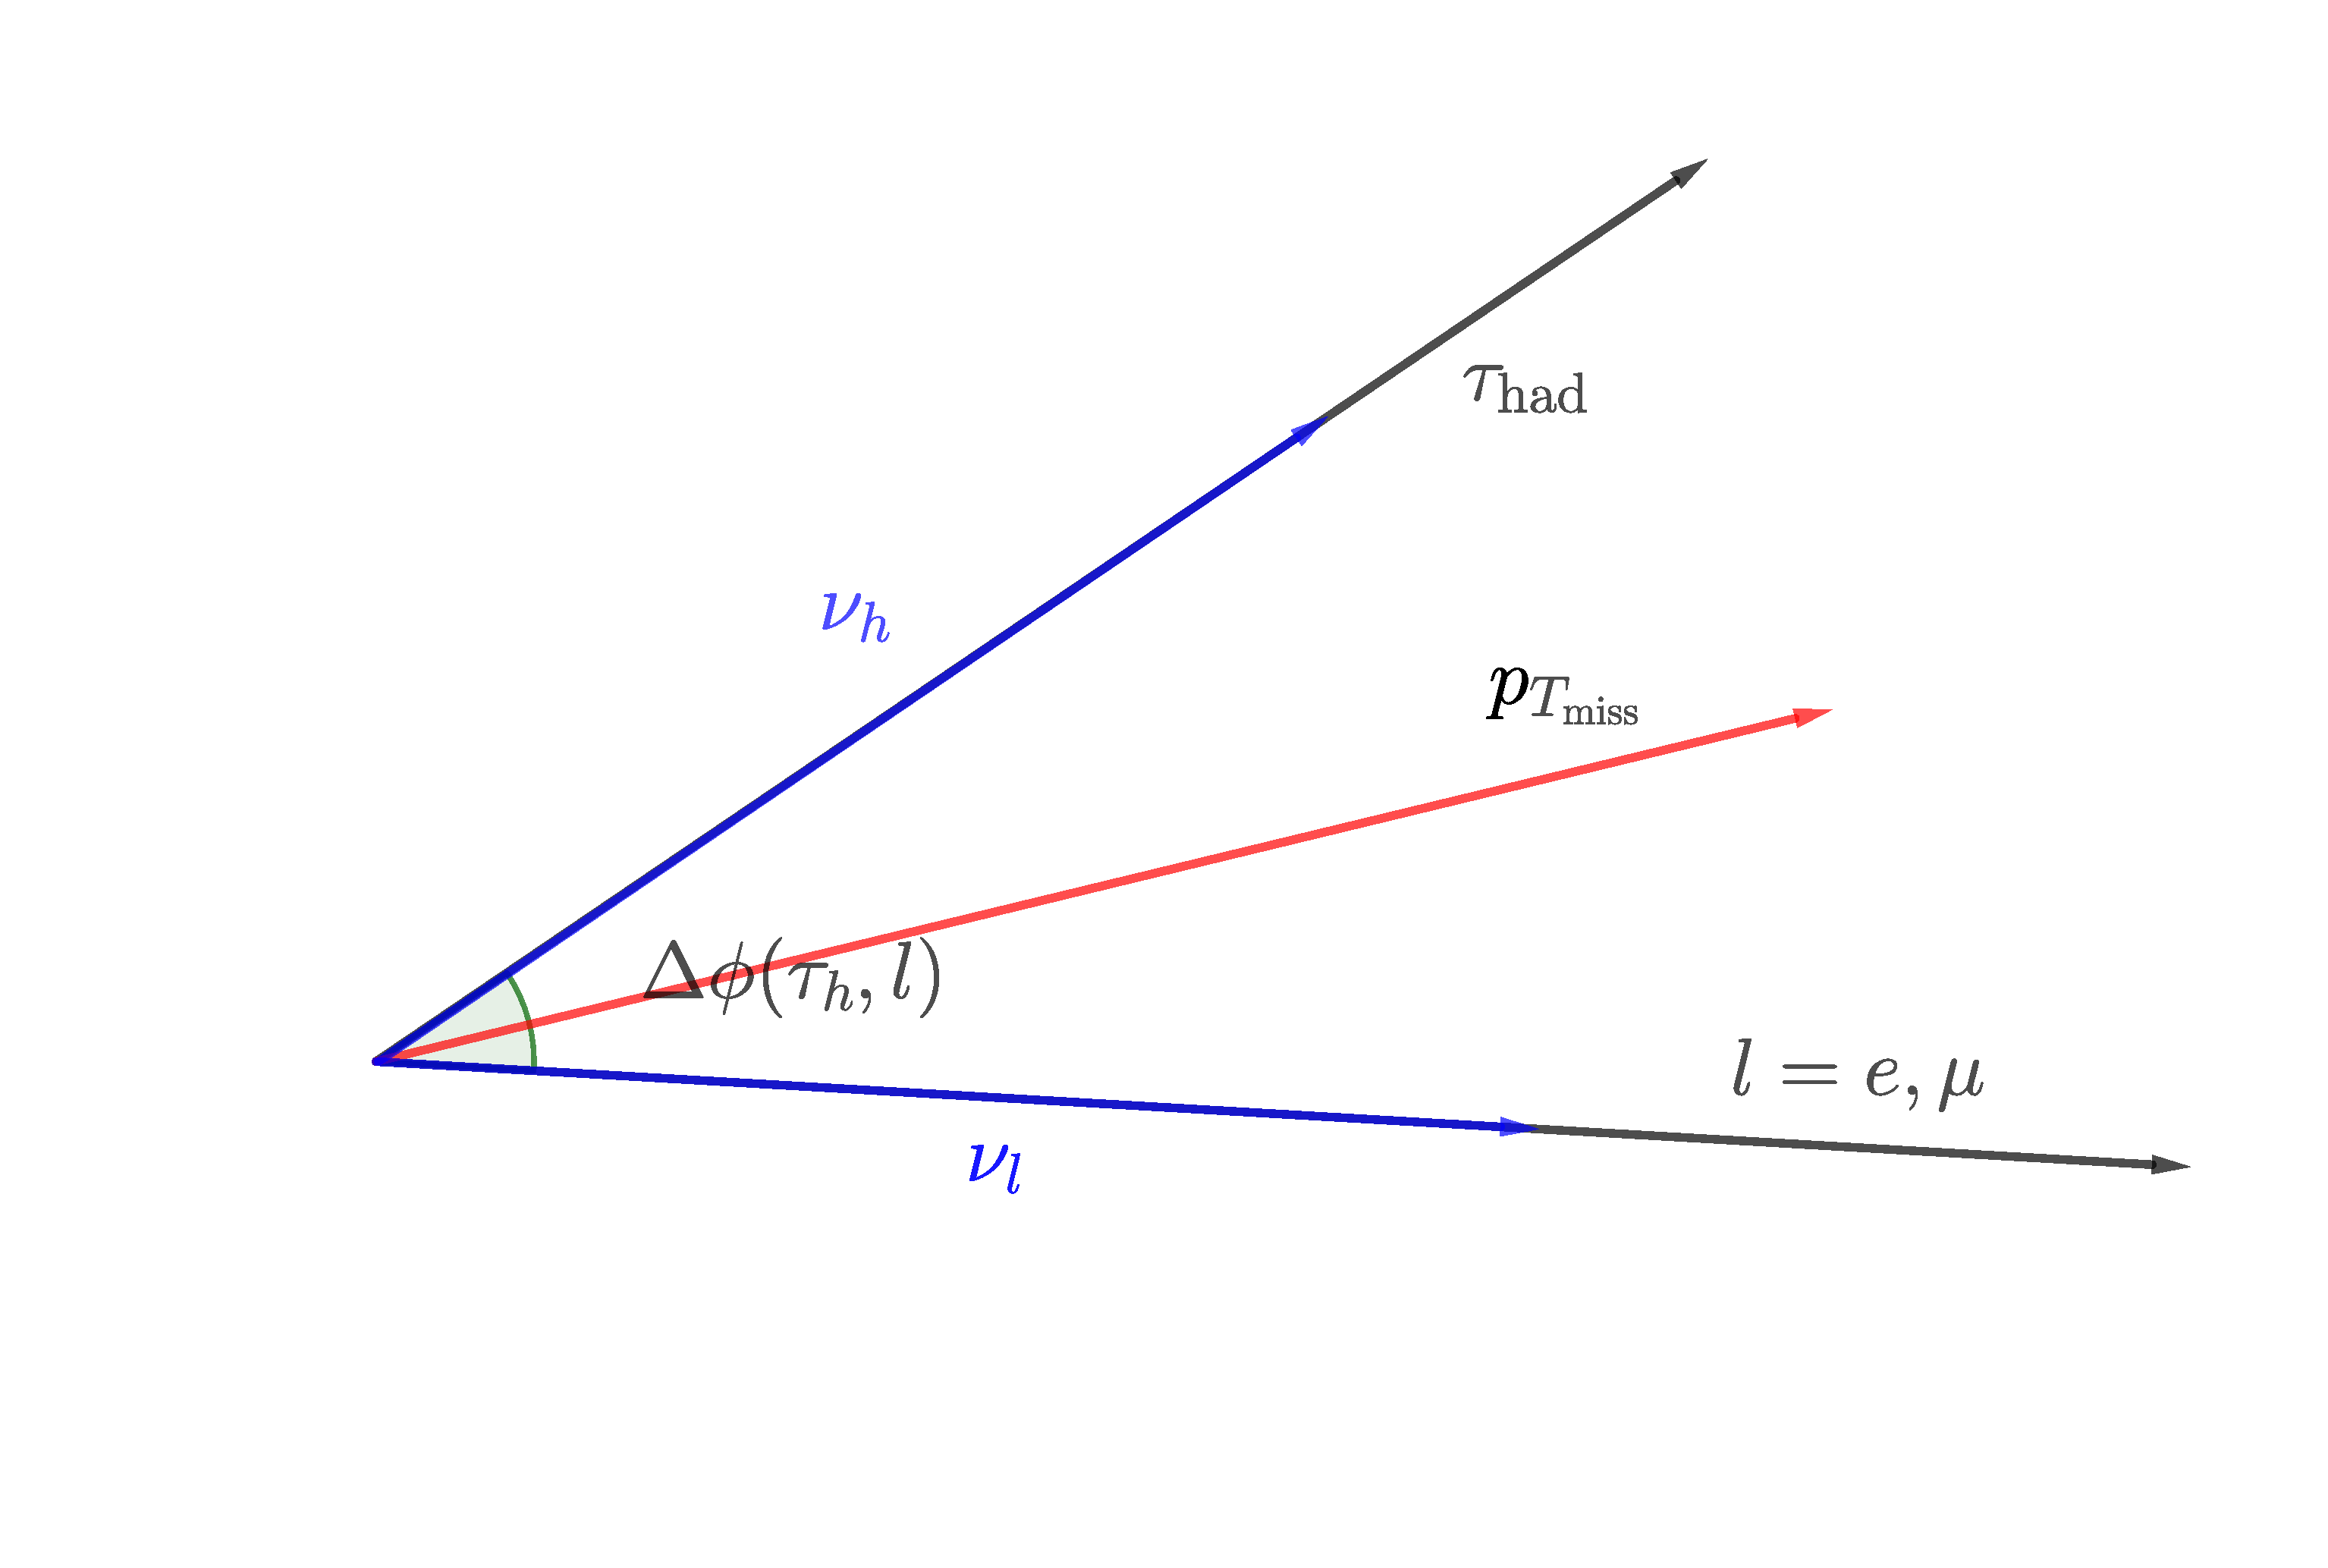
\includegraphics[width=0.45\textwidth]{figures/Fig7a}}}\hfill
	\subfloat[]{\label{Fig7b}{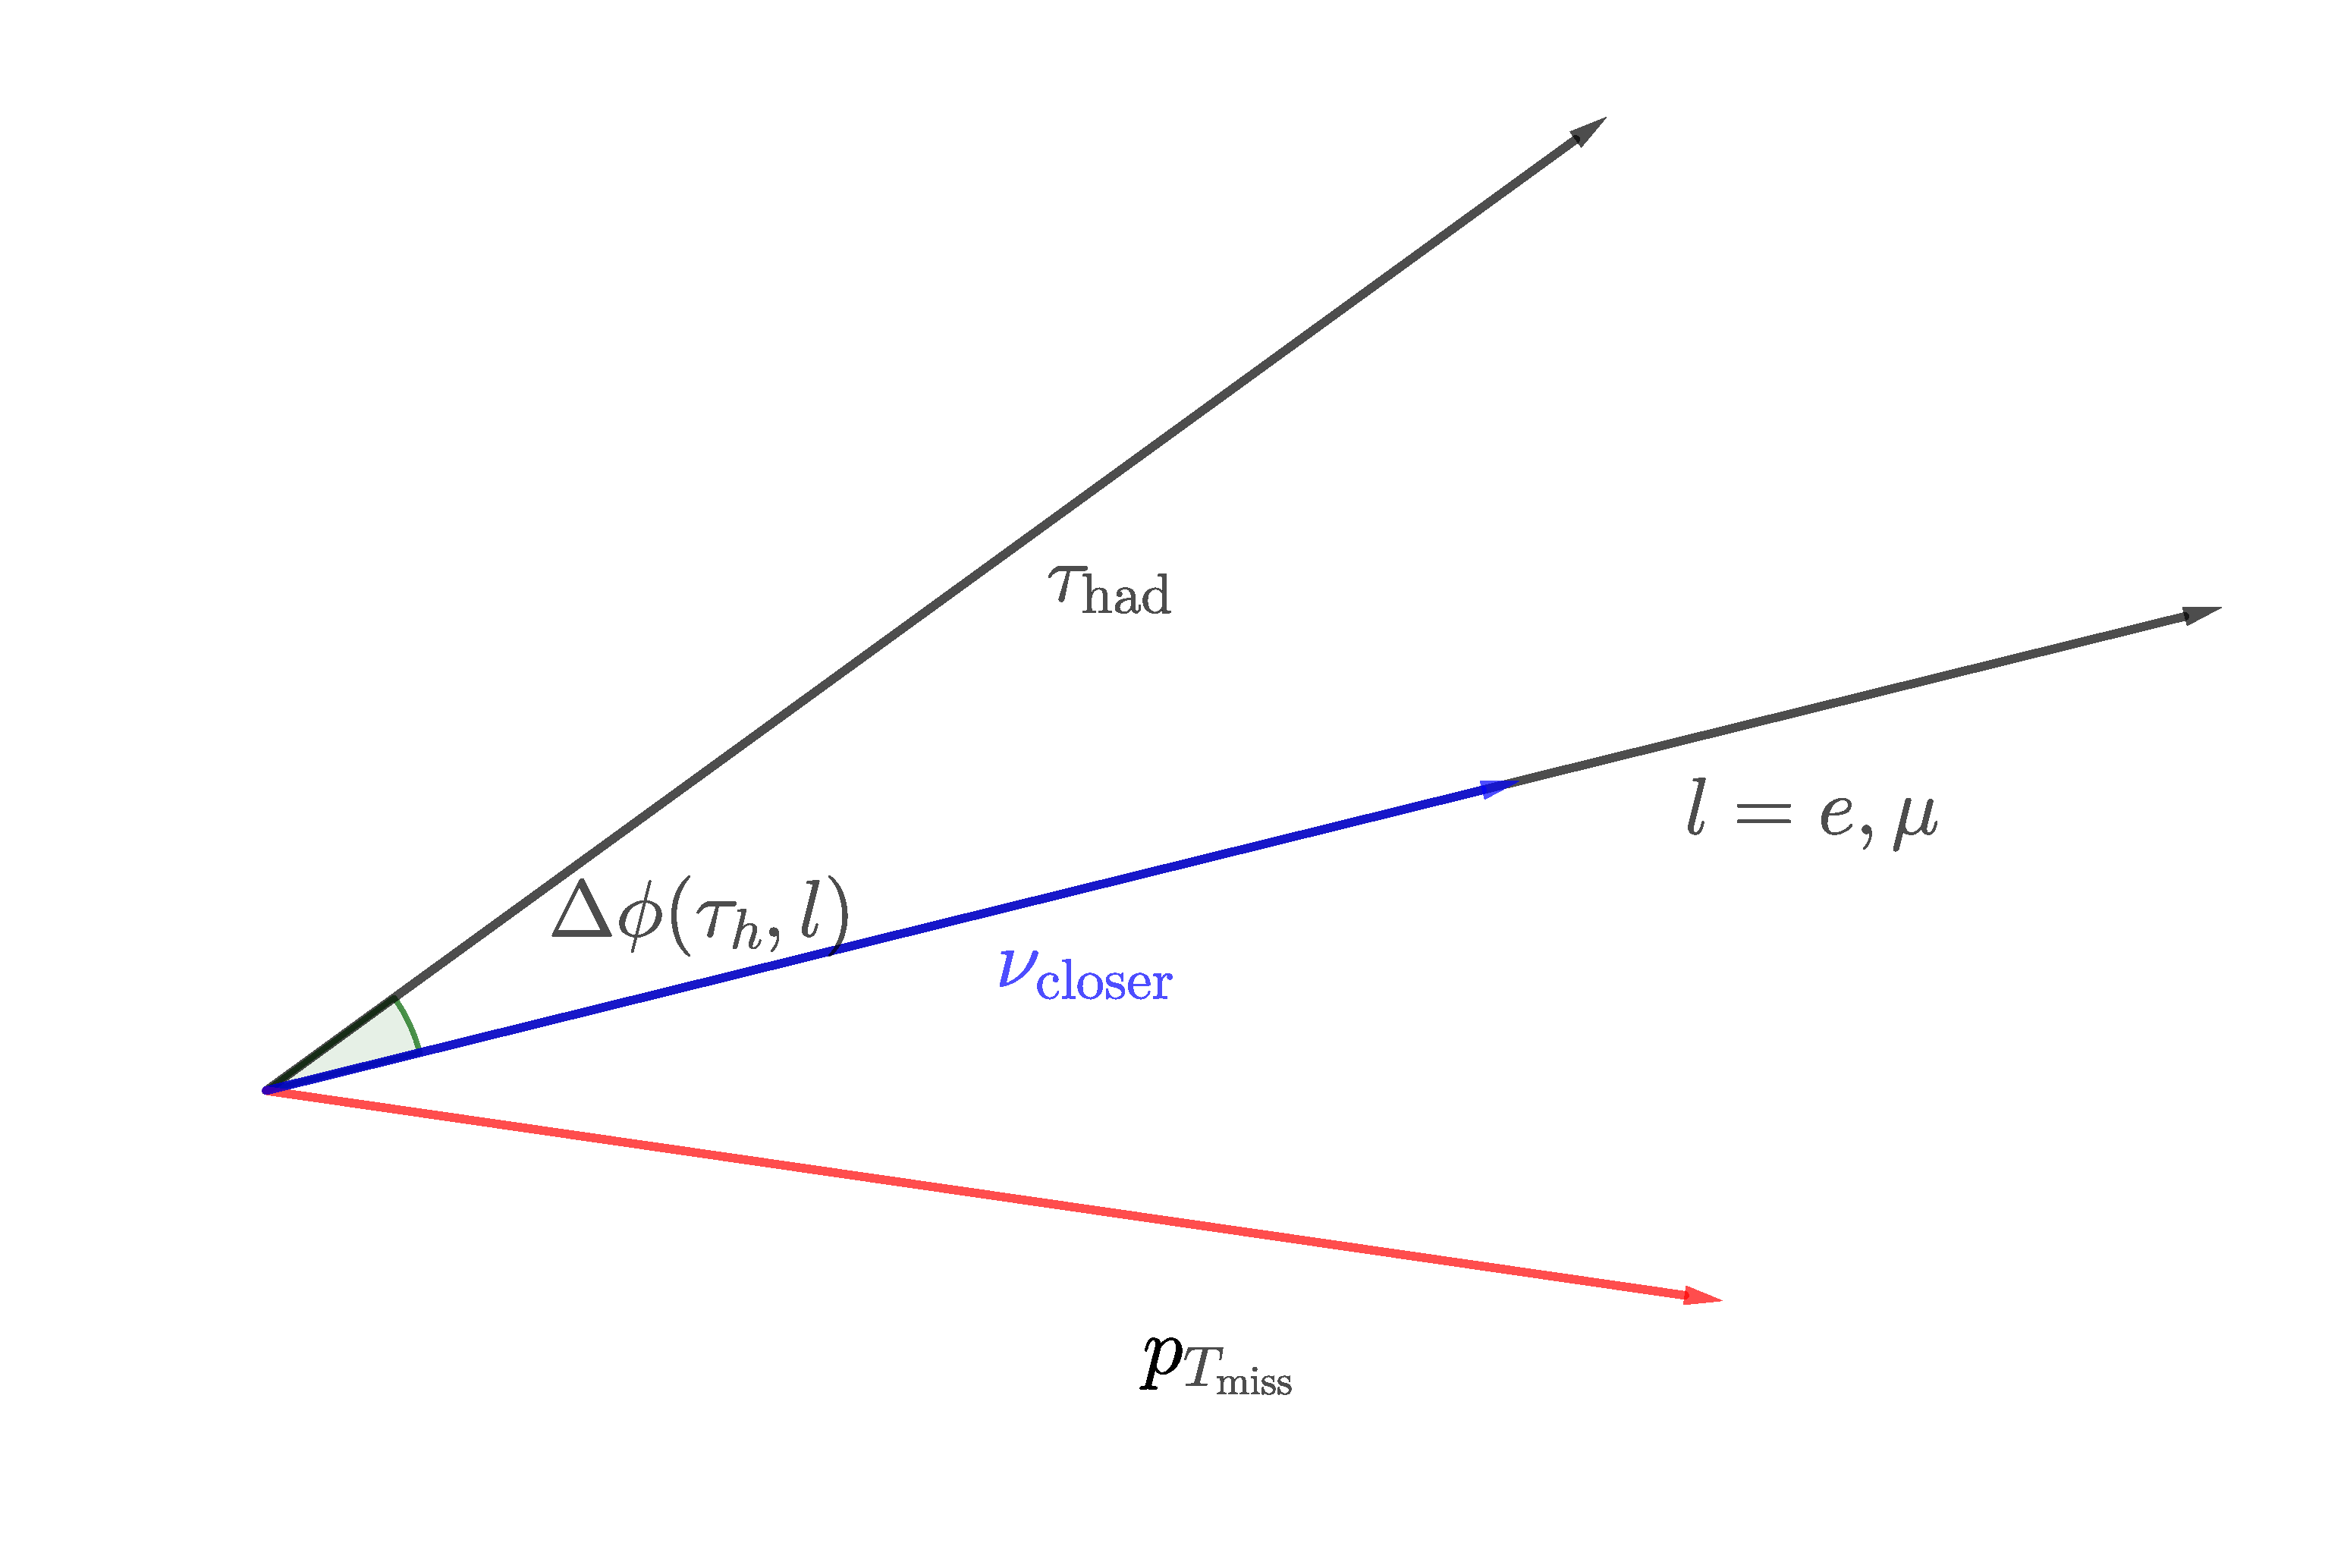
\includegraphics[width=0.45\textwidth]{figures/Fig7b}}}
	\caption{The two different types of topologies that define signal events. On the right, when the missing energy is between the visible objects two neutrinos are assumed to be responsible for all the missing energy. On the left, only one neutrino is assumed to be flying on the direction of the visible object closest to the missing energy.}
	\label{Fig7}
\end{figure}


\section{Monte Carlo Samples}

\section{The Collinear Approximation}

\section{Event Selection}